% SOURCE: submissions/d2-neurocomputing/zenodo-deposit/results/merging/RG_crossterm_alignment_ALL_REFIX20260801.json :: bundles.*.cells.g2_s{0,1,2}.{frac_cos_align_pos,rho_proj_drop} (3-seed means per bundle, 19 bundles)
% !TEX encoding = UTF-8 Unicode
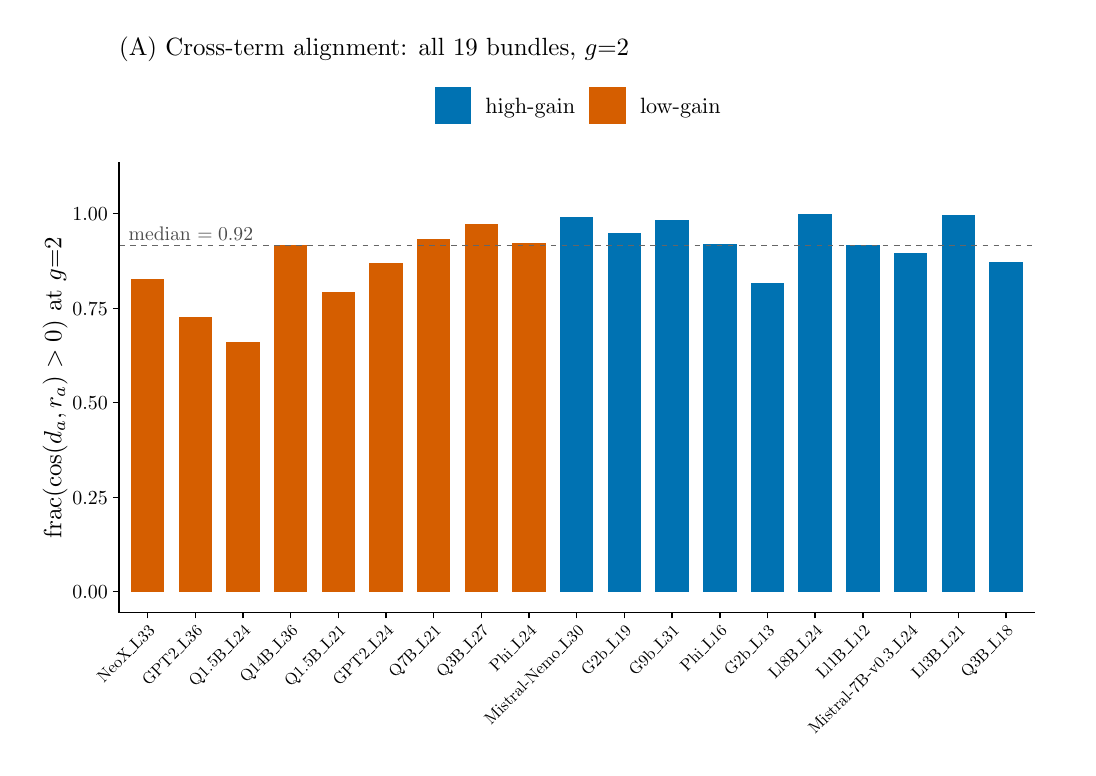
\begin{tikzpicture}[x=1pt,y=1pt]
\definecolor{fillColor}{RGB}{255,255,255}
\path[use as bounding box,fill=fillColor,fill opacity=0.00] (0,0) rectangle (375.80,260.17);
\begin{scope}
\path[clip] (  0.00,  0.00) rectangle (375.80,260.17);
\definecolor{drawColor}{RGB}{255,255,255}
\definecolor{fillColor}{RGB}{255,255,255}

\path[draw=drawColor,line width= 0.5pt,line join=round,line cap=round,fill=fillColor] (  0.00,  0.00) rectangle (375.80,260.17);
\end{scope}
\begin{scope}
\path[clip] ( 33.04, 48.95) rectangle (363.80,211.27);
\definecolor{fillColor}{RGB}{255,255,255}

\path[fill=fillColor] ( 33.04, 48.95) rectangle (363.80,211.27);
\definecolor{fillColor}{RGB}{213,94,0}

\path[fill=fillColor] ( 37.35, 56.33) rectangle ( 49.41,169.28);

\path[fill=fillColor] ( 54.58, 56.33) rectangle ( 66.64,155.61);

\path[fill=fillColor] ( 71.81, 56.33) rectangle ( 83.86,146.51);

\path[fill=fillColor] ( 89.03, 56.33) rectangle (101.09,181.58);

\path[fill=fillColor] (106.26, 56.33) rectangle (118.32,164.72);

\path[fill=fillColor] (123.49, 56.33) rectangle (135.55,175.20);

\path[fill=fillColor] (140.71, 56.33) rectangle (152.77,183.85);

\path[fill=fillColor] (157.94, 56.33) rectangle (170.00,189.32);

\path[fill=fillColor] (175.17, 56.33) rectangle (187.23,182.49);
\definecolor{fillColor}{RGB}{0,114,178}

\path[fill=fillColor] (192.39, 56.33) rectangle (204.45,191.59);

\path[fill=fillColor] (209.62, 56.33) rectangle (221.68,186.13);

\path[fill=fillColor] (226.85, 56.33) rectangle (238.91,190.68);

\path[fill=fillColor] (244.08, 56.33) rectangle (256.14,182.03);

\path[fill=fillColor] (261.30, 56.33) rectangle (273.36,167.91);

\path[fill=fillColor] (278.53, 56.33) rectangle (290.59,192.96);

\path[fill=fillColor] (295.76, 56.33) rectangle (307.82,181.58);

\path[fill=fillColor] (312.98, 56.33) rectangle (325.04,178.84);

\path[fill=fillColor] (330.21, 56.33) rectangle (342.27,192.51);

\path[fill=fillColor] (347.44, 56.33) rectangle (359.50,175.65);
\definecolor{drawColor}{gray}{0.40}

\path[draw=drawColor,line width= 0.3pt,dash pattern=on 2pt off 2pt ,line join=round] ( 33.04,181.58) -- (363.80,181.58);
\definecolor{drawColor}{gray}{0.30}

\node[text=drawColor,anchor=base west,inner sep=0pt, outer sep=0pt, scale=  0.71] at ( 36.49,183.22) {median $= 0.92$};
\end{scope}
\begin{scope}
\path[clip] (  0.00,  0.00) rectangle (375.80,260.17);
\definecolor{drawColor}{RGB}{0,0,0}

\path[draw=drawColor,line width= 0.5pt,line join=round,line cap=rect] ( 33.04, 48.95) --
	( 33.04,211.27);
\end{scope}
\begin{scope}
\path[clip] (  0.00,  0.00) rectangle (375.80,260.17);
\definecolor{drawColor}{RGB}{0,0,0}

\node[text=drawColor,anchor=base east,inner sep=0pt, outer sep=0pt, scale=  0.72] at ( 28.99, 53.85) {0.00};

\node[text=drawColor,anchor=base east,inner sep=0pt, outer sep=0pt, scale=  0.72] at ( 28.99, 88.01) {0.25};

\node[text=drawColor,anchor=base east,inner sep=0pt, outer sep=0pt, scale=  0.72] at ( 28.99,122.17) {0.50};

\node[text=drawColor,anchor=base east,inner sep=0pt, outer sep=0pt, scale=  0.72] at ( 28.99,156.32) {0.75};

\node[text=drawColor,anchor=base east,inner sep=0pt, outer sep=0pt, scale=  0.72] at ( 28.99,190.48) {1.00};
\end{scope}
\begin{scope}
\path[clip] (  0.00,  0.00) rectangle (375.80,260.17);
\definecolor{drawColor}{RGB}{0,0,0}

\path[draw=drawColor,line width= 0.5pt,line join=round] ( 30.79, 56.33) --
	( 33.04, 56.33);

\path[draw=drawColor,line width= 0.5pt,line join=round] ( 30.79, 90.49) --
	( 33.04, 90.49);

\path[draw=drawColor,line width= 0.5pt,line join=round] ( 30.79,124.64) --
	( 33.04,124.64);

\path[draw=drawColor,line width= 0.5pt,line join=round] ( 30.79,158.80) --
	( 33.04,158.80);

\path[draw=drawColor,line width= 0.5pt,line join=round] ( 30.79,192.96) --
	( 33.04,192.96);
\end{scope}
\begin{scope}
\path[clip] (  0.00,  0.00) rectangle (375.80,260.17);
\definecolor{drawColor}{RGB}{0,0,0}

\path[draw=drawColor,line width= 0.5pt,line join=round,line cap=rect] ( 33.04, 48.95) --
	(363.80, 48.95);
\end{scope}
\begin{scope}
\path[clip] (  0.00,  0.00) rectangle (375.80,260.17);
\definecolor{drawColor}{RGB}{0,0,0}

\path[draw=drawColor,line width= 0.5pt,line join=round] ( 43.38, 46.70) --
	( 43.38, 48.95);

\path[draw=drawColor,line width= 0.5pt,line join=round] ( 60.61, 46.70) --
	( 60.61, 48.95);

\path[draw=drawColor,line width= 0.5pt,line join=round] ( 77.84, 46.70) --
	( 77.84, 48.95);

\path[draw=drawColor,line width= 0.5pt,line join=round] ( 95.06, 46.70) --
	( 95.06, 48.95);

\path[draw=drawColor,line width= 0.5pt,line join=round] (112.29, 46.70) --
	(112.29, 48.95);

\path[draw=drawColor,line width= 0.5pt,line join=round] (129.52, 46.70) --
	(129.52, 48.95);

\path[draw=drawColor,line width= 0.5pt,line join=round] (146.74, 46.70) --
	(146.74, 48.95);

\path[draw=drawColor,line width= 0.5pt,line join=round] (163.97, 46.70) --
	(163.97, 48.95);

\path[draw=drawColor,line width= 0.5pt,line join=round] (181.20, 46.70) --
	(181.20, 48.95);

\path[draw=drawColor,line width= 0.5pt,line join=round] (198.42, 46.70) --
	(198.42, 48.95);

\path[draw=drawColor,line width= 0.5pt,line join=round] (215.65, 46.70) --
	(215.65, 48.95);

\path[draw=drawColor,line width= 0.5pt,line join=round] (232.88, 46.70) --
	(232.88, 48.95);

\path[draw=drawColor,line width= 0.5pt,line join=round] (250.11, 46.70) --
	(250.11, 48.95);

\path[draw=drawColor,line width= 0.5pt,line join=round] (267.33, 46.70) --
	(267.33, 48.95);

\path[draw=drawColor,line width= 0.5pt,line join=round] (284.56, 46.70) --
	(284.56, 48.95);

\path[draw=drawColor,line width= 0.5pt,line join=round] (301.79, 46.70) --
	(301.79, 48.95);

\path[draw=drawColor,line width= 0.5pt,line join=round] (319.01, 46.70) --
	(319.01, 48.95);

\path[draw=drawColor,line width= 0.5pt,line join=round] (336.24, 46.70) --
	(336.24, 48.95);

\path[draw=drawColor,line width= 0.5pt,line join=round] (353.47, 46.70) --
	(353.47, 48.95);
\end{scope}
\begin{scope}
\path[clip] (  0.00,  0.00) rectangle (375.80,260.17);
\definecolor{drawColor}{RGB}{0,0,0}

\node[text=drawColor,rotate= 45.00,anchor=base east,inner sep=0pt, outer sep=0pt, scale=  0.60] at ( 46.30, 41.98) {NeoX\_L33};

\node[text=drawColor,rotate= 45.00,anchor=base east,inner sep=0pt, outer sep=0pt, scale=  0.60] at ( 63.53, 41.98) {GPT2\_L36};

\node[text=drawColor,rotate= 45.00,anchor=base east,inner sep=0pt, outer sep=0pt, scale=  0.60] at ( 80.76, 41.98) {Q1.5B\_L24};

\node[text=drawColor,rotate= 45.00,anchor=base east,inner sep=0pt, outer sep=0pt, scale=  0.60] at ( 97.98, 41.98) {Q14B\_L36};

\node[text=drawColor,rotate= 45.00,anchor=base east,inner sep=0pt, outer sep=0pt, scale=  0.60] at (115.21, 41.98) {Q1.5B\_L21};

\node[text=drawColor,rotate= 45.00,anchor=base east,inner sep=0pt, outer sep=0pt, scale=  0.60] at (132.44, 41.98) {GPT2\_L24};

\node[text=drawColor,rotate= 45.00,anchor=base east,inner sep=0pt, outer sep=0pt, scale=  0.60] at (149.67, 41.98) {Q7B\_L21};

\node[text=drawColor,rotate= 45.00,anchor=base east,inner sep=0pt, outer sep=0pt, scale=  0.60] at (166.89, 41.98) {Q3B\_L27};

\node[text=drawColor,rotate= 45.00,anchor=base east,inner sep=0pt, outer sep=0pt, scale=  0.60] at (184.12, 41.98) {Phi\_L24};

\node[text=drawColor,rotate= 45.00,anchor=base east,inner sep=0pt, outer sep=0pt, scale=  0.60] at (201.35, 41.98) {Mistral-Nemo\_L30};

\node[text=drawColor,rotate= 45.00,anchor=base east,inner sep=0pt, outer sep=0pt, scale=  0.60] at (218.57, 41.98) {G2b\_L19};

\node[text=drawColor,rotate= 45.00,anchor=base east,inner sep=0pt, outer sep=0pt, scale=  0.60] at (235.80, 41.98) {G9b\_L31};

\node[text=drawColor,rotate= 45.00,anchor=base east,inner sep=0pt, outer sep=0pt, scale=  0.60] at (253.03, 41.98) {Phi\_L16};

\node[text=drawColor,rotate= 45.00,anchor=base east,inner sep=0pt, outer sep=0pt, scale=  0.60] at (270.25, 41.98) {G2b\_L13};

\node[text=drawColor,rotate= 45.00,anchor=base east,inner sep=0pt, outer sep=0pt, scale=  0.60] at (287.48, 41.98) {Ll8B\_L24};

\node[text=drawColor,rotate= 45.00,anchor=base east,inner sep=0pt, outer sep=0pt, scale=  0.60] at (304.71, 41.98) {Ll1B\_L12};

\node[text=drawColor,rotate= 45.00,anchor=base east,inner sep=0pt, outer sep=0pt, scale=  0.60] at (321.94, 41.98) {Mistral-7B-v0.3\_L24};

\node[text=drawColor,rotate= 45.00,anchor=base east,inner sep=0pt, outer sep=0pt, scale=  0.60] at (339.16, 41.98) {Ll3B\_L21};

\node[text=drawColor,rotate= 45.00,anchor=base east,inner sep=0pt, outer sep=0pt, scale=  0.60] at (356.39, 41.98) {Q3B\_L18};
\end{scope}
\begin{scope}
\path[clip] (  0.00,  0.00) rectangle (375.80,260.17);
\definecolor{drawColor}{RGB}{0,0,0}

\node[text=drawColor,rotate= 90.00,anchor=base,inner sep=0pt, outer sep=0pt, scale=  0.90] at ( 12.20,130.11) {frac($\cos(d_a, r_a)>0$) at $g{=}2$};
\end{scope}
\begin{scope}
\path[clip] (  0.00,  0.00) rectangle (375.80,260.17);
\definecolor{fillColor}{RGB}{255,255,255}

\path[fill=fillColor] (141.95,220.27) rectangle (254.90,243.72);
\end{scope}
\begin{scope}
\path[clip] (  0.00,  0.00) rectangle (375.80,260.17);
\definecolor{fillColor}{RGB}{255,255,255}

\path[fill=fillColor] (146.45,224.77) rectangle (160.90,239.22);
\definecolor{fillColor}{RGB}{0,114,178}

\path[fill=fillColor] (147.03,225.35) rectangle (160.32,238.64);
\end{scope}
\begin{scope}
\path[clip] (  0.00,  0.00) rectangle (375.80,260.17);
\definecolor{fillColor}{RGB}{255,255,255}

\path[fill=fillColor] (202.34,224.77) rectangle (216.79,239.22);
\definecolor{fillColor}{RGB}{213,94,0}

\path[fill=fillColor] (202.92,225.35) rectangle (216.21,238.64);
\end{scope}
\begin{scope}
\path[clip] (  0.00,  0.00) rectangle (375.80,260.17);
\definecolor{drawColor}{RGB}{0,0,0}

\node[text=drawColor,anchor=base west,inner sep=0pt, outer sep=0pt, scale=  0.80] at (165.40,229.24) {high-gain};
\end{scope}
\begin{scope}
\path[clip] (  0.00,  0.00) rectangle (375.80,260.17);
\definecolor{drawColor}{RGB}{0,0,0}

\node[text=drawColor,anchor=base west,inner sep=0pt, outer sep=0pt, scale=  0.80] at (221.29,229.24) {low-gain};
\end{scope}
\begin{scope}
\path[clip] (  0.00,  0.00) rectangle (375.80,260.17);
\definecolor{drawColor}{RGB}{0,0,0}

\node[text=drawColor,anchor=base west,inner sep=0pt, outer sep=0pt, scale=  0.90] at ( 33.04,249.97) {(A) Cross-term alignment: all 19 bundles, $g{=}2$};
\end{scope}
\end{tikzpicture}
